
We propose a \textit{design pattern} for building query processing systems,
with the goal of evolving query processing system's architecture from monolithic and static to modular and flexible.
Traditional static query processing systems are not able to cater to the needs of modern applications in which users and
data are geo-distributed across the globe.
Our vision is to enable query processing systems that are designed and deployed on a case-by-case basis,
with the workload characteristics, data and access distribution patterns, and requirements of specific applications in
mind.
As a first step towards this vision, we focus on the \texit{mechanisms} required for enabling a flexible and configurable
query processing system architecture.

\medskip

The key idea for the proposed design pattern \textit{assembly-based modularity}.
The query processing system's architecture is modular:
it is constructed by interconnecting composable building blocks
that encapsulate components of a traditional query processing system such as indexes, materialized views,
and caches, as well as relational operators such as filters, aggregations, and joins.
Modularity translates design decisions about the use of derived state to which building blocks are used and how they are
interconnected.
For example, adding a caching layer to an existing system can be done by extending an existing query system architecture
with additional building blocks.

Moreover, modularity enables configurable placement.
The components of a modular architecture, as opposed to a monolithic one,
can be decoupled from the storage tier, and flexibly placed across the system infrastructure.


\section{Overview: a modular query processing architecture}

According to the design pattern that we propose,
a query processing system is a composition of building blocks that encapsulate query processing tasks, called
Query Processing Units (QPUs).

A QPU can be viewed as a microservice responsible for receiving and processing queries.
It receives one or more input streams, performs a computation over these streams, and emits an output stream.
This is initiated when the QPU receives a query request.

QPUs can implement relational query processing operators.
For example, a QPU that implements a join operator receives the records of two tables as input streams,
and emits the result of the join operation as the output stream.

Moreover, QPUs can implement derived state structures such as indexes, materialized views and caches.
For example, a QPU that implements a secondary index on a table receives notifications for updates to that table as an
input stream and builds the secondary index, which it stores as internal state.
When it receives a query request, it reads from the index and emits the result as an output stream.

Our key insight is that both QPUs that implement streaming relational operators and those that implement derived state structures
can be generalized to a system component with common semantics.

QPUs are organized in a directed acyclic graph:
a QPU can send query requests to other QPUs it has outgoing connections to in the graph (downstream neighbors)
Base data are the leaves of the graph (nodes with only incoming edges),
and client queries enter the graph through its root nodes (nodes with outgoing edges).

When a QPU receives a query, it can process it by reading from its internal state, it can initiate input streams
by sending query requests to its some of its downstream neighbors and produce query results using these streams,
or a combination of the two.
This process is recursively performed at each downstream QPU, creating a query execution tree.


\subsection{The Query Processing Unit abstraction}

The key property required by query processing unit to effectively serve as building blocks of the modular query
processing systems is composability:
QPUs should be able to be interconnected in various topologies, and interoperate in the execution of query processing tasks.

To achieve this, we define a common set of properties that any query processing unit should conform to.
This properties include a common interface for receiving query request, and common the interaction semantics among QPUs.
We call this set of properties the query processing unit \textit{abstraction}.
Using object-oriented programming terminology, the QPU abstraction can be viewed as an \textit{abstract class}
that defines a set of methods, but does not include their implementation.
Implementations of the QPU abstraction define \textit{QPU classes} with specific functionalities,
such as join or index QPU classes.
Using the object-oriented programming analogy, QPU classes can be viewed as classes that implement the QPU
abstract class.
Finally, specific \textit{QPU instances} can be viewed as objects of a specific QPU class, for example a index QPU that
indexes the attribute $predominantColor$ of a table $photoAlbum$.
The building blocks of a modular query processing system are QPU instances.

In the rest of this thesis we use the terms query processing unit, QPU, and unit interchangeably to refer to QPU instances.

\bigskip

More specifically, the query processing unit abstraction defines a \textit{system component} with the following properties:

\begin{figure}[t]
  \centering
    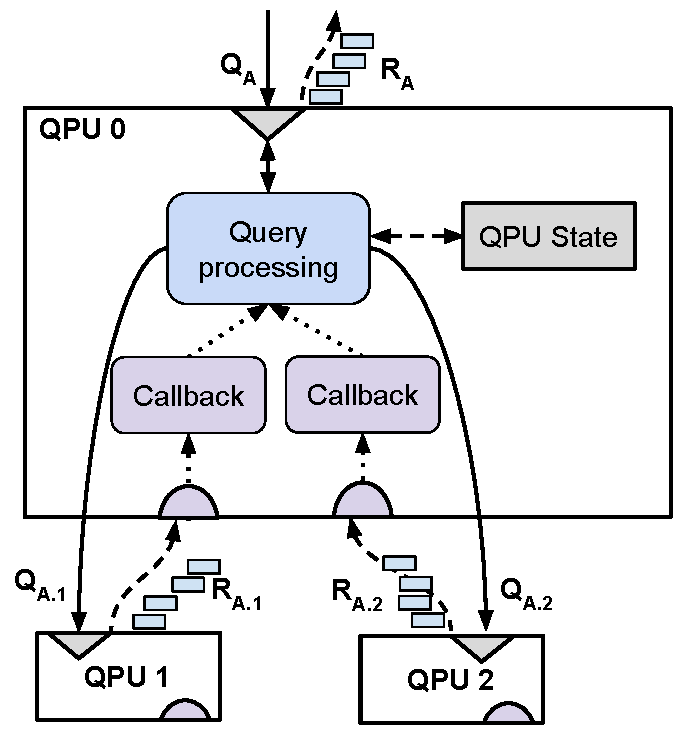
\includegraphics[width=0.5\textwidth]{./figures/design_pattern/qpu_abstraction.pdf}
  \caption{A conceptual depiction the QPU abstraction.}
  \label{fig:qpu_abstraction}
\end{figure}

% \subsubsection{Query interface}
\medskip

\noindent
\textbf{Query interface.}
Every QPU exposes an interface for receiving query requests.
While this interface is common among all QPUs, QPU classes and specific QPU instances restrict the set of queries
that they can serve.
For example, a QPU may only serve queries about a specific database table.
As a result, QPUs can be though of as microservices that serve queries

The QPU's query interface has \textit{streaming semantics}.
An invocation of the interface establishes between the QPU and caller:
the QPU sends query result entries as stream records; the caller can send control messages such as acknowledgements.
We present the query interface in more detail in section \todo{ref}.

The query interface can be invoked by other query processing units.
This is how QPUs interoperate and forms the basis of the query processing system's computation model \todo{ref}.
We call the act of a $QPU_a$ invoking the query interface of a $QPU_b$, a \textit{downstream query}.

\medskip

\noindent
\textbf{Query processing function}
Every QPU implements a function that is called when its query interface is invoked, and is responsible for processing
the given query and writing to the query result stream.

The implementation of this computation is may differ between QPU classes.

Two capabilities are available for the implementation of the query processing function:
accessing the QPU's state, and initiating input streams by sending query requests to downstream neighbors.

\medskip

\noindent
\textbf{State}
A QPU maintains three types of state:
\begin{itemize}

\item \textbf{Query processing state.}
This state can represent derived derived state, such as an index, a materialized view, or cache,
it can be used for intermediate results, for example \todo{in streaming join computation?}.
Some QPUs classes, such as a filter operator may not use query processing at all.
A QPU can either maintain state, or be stateless.
Stateful QPUs can express query processing tasks such as indexing (in which case the state is an indexing data
structure), caching, and aggregation computations.
Stateless QPUs can express tasks such as filtering and projections.

\item \textbf{Configuration state.}
This type of state is composed of configuration parameters, such as the endpoint of its downstream neighbors.
\todo{ref}

\item \textbf{Downstream neighbors metadata.}
Each QPU maintains metadata that represent information about its downstream neighbors, such as their QPU class,
and their capabilities \todo{ref}.
These metadata is used during query processing for generating downstream query requests \todo{ref}.
\end{itemize}

\medskip

\noindent
\textbf{Input stream callback function.}
Each QPU implements a callback function that is called for each record received through an input stream.

\bigskip

A conceptual depiction of the query processing unit abstraction is shown in Figure~\ref{fig:qpu_abstraction}.
When the QPU's query API is called, a response stream ($R_A$) is established between the unit and the client, and
the unit's query processing computation is invoked.
The query processing computation can read the QPU's state, and can perform downstream queries to other units.
For each downstream query, a corresponding stream is established ($Q_{A.1}$ and $Q_{A.2}$).
When a record is received from one of the streams, the QPU's callback computation is invoked.
Each callback computation processes the received record, and returns the result to the query processing computation.
Upon receiving a result from the callback, the query processing computation can write to the QPU's
state and potentially send a computed query result through the response stream.


\subsection{Query API}
% Define the ``query'' API method (arguments, streaming semantics).

% The QPU defines a ``query processing'' function that is invoked each time the
% QPU receives a query.

% Different QPU types use different implementations of the ``query processing''
% function.

\subsubsection{Streaming query response}
% Each invocation of a QPU's ``query'' API returns a stream handler.
% The caller uses the stream handler to get the query responses as stream records.

% The QPU defines a ``callback'' function that is invoked each time the QPU
% receives a stream record.

% Different QPU types use different implementations of the ``callback''
% function.

\subsection{QPU State}
% Describe the different parts of the QPU state and their indented functionality.

\subsubsection{Query processing state}
% This is the main part of the state (implements index and cache data structures).
% It is read to process queries, and is updated using stream records from other
% QPUs.
\subsubsection{Configuration state}
% This is the part of the state that defines the QPU's behavior (includes its type
% and neighborhood).
% Passed as argument during initialization.

\subsubsection{Local graph view state}
% This is the part of the state that describes the QPU's knowledge/view of the
% sub-graphs it is connected to.
% It is initialized using the ``getConfig'' API method.

\section{QPU classes (overview)}
\label{sec:qpu_classes}

% As described earlier, the QPU abstraction works as a ``blueprint''.
% It specifies a communication and execution protocol that QPUs must conform to.
% However, there can be different instantiations of this specification.
% We term these instantiations of the QPU abstraction, classes.

% More specifically, each QPU class defines:
% \begin{itemize}
%   \item The query processing state of the units is this class.
%   \item Their query processing and callback functions.
% \end{itemize}

% We categorize QPU classes in three distinct families:
% \begin{itemize}
%   \item \textbf{Stateful QPUs}. QPU classes of this family maintain internal
%   query processing state and use it to process queries.
%   Examples include index, cache, and materialized view QPUs.
%   \item \textbf{Stateless QPUs}. QPU classes of this family do no maintain
%   internal query processing state (or maintain only intermediate state).
%   Stateless (or Functional ?) QPUs process queries by performing computation on
%   incoming streams (they initiate streams by sending queries to other QPUs.)
%   Examples include filter, join, and aggregation QPUs.
%   \item \textbf{Routing QPUs}. Stateful and stateless QPUs can only have a
%   single outgoing (child) connection in the QPU graph.
%   TODO: QPU graph has not been defined until point. Define-before-reference.
%   Routing QPUs have multiple outgoing connections.
%   They are responsible for re-writing incoming to queries to sub-queries,
%   sending them to the appropriate child QPUs, and merging the responses to a
%   single outgoing response stream.
%   Routing QPUs can be used for example to build sharded indexes by composing
%   multiple index QPUs.
% \end{itemize}

\section{QPU Composition: Constructing QPU-based query engines}
Here, describe how query engines are constructed using instances of QPU classes.

A query engine is a directed acyclic graph (why?) with QPUs as nodes.

Describe the QPU-specific topology properties that the graph must satisfy in
order to be functional:
\begin{itemize}
  \item All leaves must be QPUs of the datastore driver class.
  Also, datastore driver QPUs cannot be nodes other than leaves.
  \item TODO
\end{itemize}

\section{Computation Model}
Describe the bidirectional data-flow computation.
\begin{itemize}
  \item Control messages (queries) flow downwards.
  \item Responses flow upwards through the sub-graph defined by the control
  (each query establishes a sub-graph - actually a tree - to be used by that
  particular query);
  \item Updates (independently) also flow upwards.
\end{itemize}


\section{The consistency guarantees of QPU-based query engines}
TODO: What mechanism are needed so that QPUs can guarantee internal consistency?
What about session consistency guarantees?

\subsection{Discussion}
It is known that query execution can be represented as a tree.
Base data are at the tree's leaves, tree nodes are relational operator such
as filter, joins and aggregations, and query result are at the root of the tree.
Each operator receives an input stream of records, performs a transformation on the, and emits a output stream of record.
This results to a data-flow computation in which data items flow upwards through the tree and are progressively transformed
to the query execution results.

Computation tasks vs architecture components